\chapter{Metric Improvements} \label{ch:metrics}

The work presented in this chapter is an extension of the metric gathering work described in chapter 3.  In this chapter we discuss changes to the metric gathering approach, an adaptation of another cognitive workload metric, and changes to the metric calculations.

\section{Metric Gathering Approach}

There are two general approaches for extracting simulation data into meaningful metrics: capture and report all raw data and use post processing to extract the metrics or capture only that data which we know to represent meaningful metrics and ignore the rest.  The first approach is valuable in that the volume of data has the potential to provide many first, second, and third order metrics which are not visible when sampling.  For example other researchers on this project are using trends in the data to help summarize the data at a higher level of abstraction.  Unfortunately the high volume of data also makes it more difficult to find meaningful metrics.  The sample approach simplifies the collection of specific metrics but it may make it more difficult to compare multiple metrics if the raw data which connects those metrics was not captured.

For this thesis we present a mixed data extraction approach.  Figure~\ref{fig:metric_gathering} shows the \textit{first in last out} metric stack which was used to obtain more accurate metric data from the labeled state transition system hierarchy.  For each time step in the simulation the Simulator will ask the Team for metrics, which triggers a chain of metric requests down to the transition level.  When it is time for a component to sample the raw data, it will select a sample of the raw data and pass it to its parent.  The parent then selects its own sample data from the available raw data and the sample returned by its child.  This allows the component to perform pre-processing on the raw data, which is much easier to accomplish while the data is still within the original context.  It also captures a unified timeline for all of the metrics, which helps to tie the metrics together.  

\begin{figure}[h]
\begin{center}
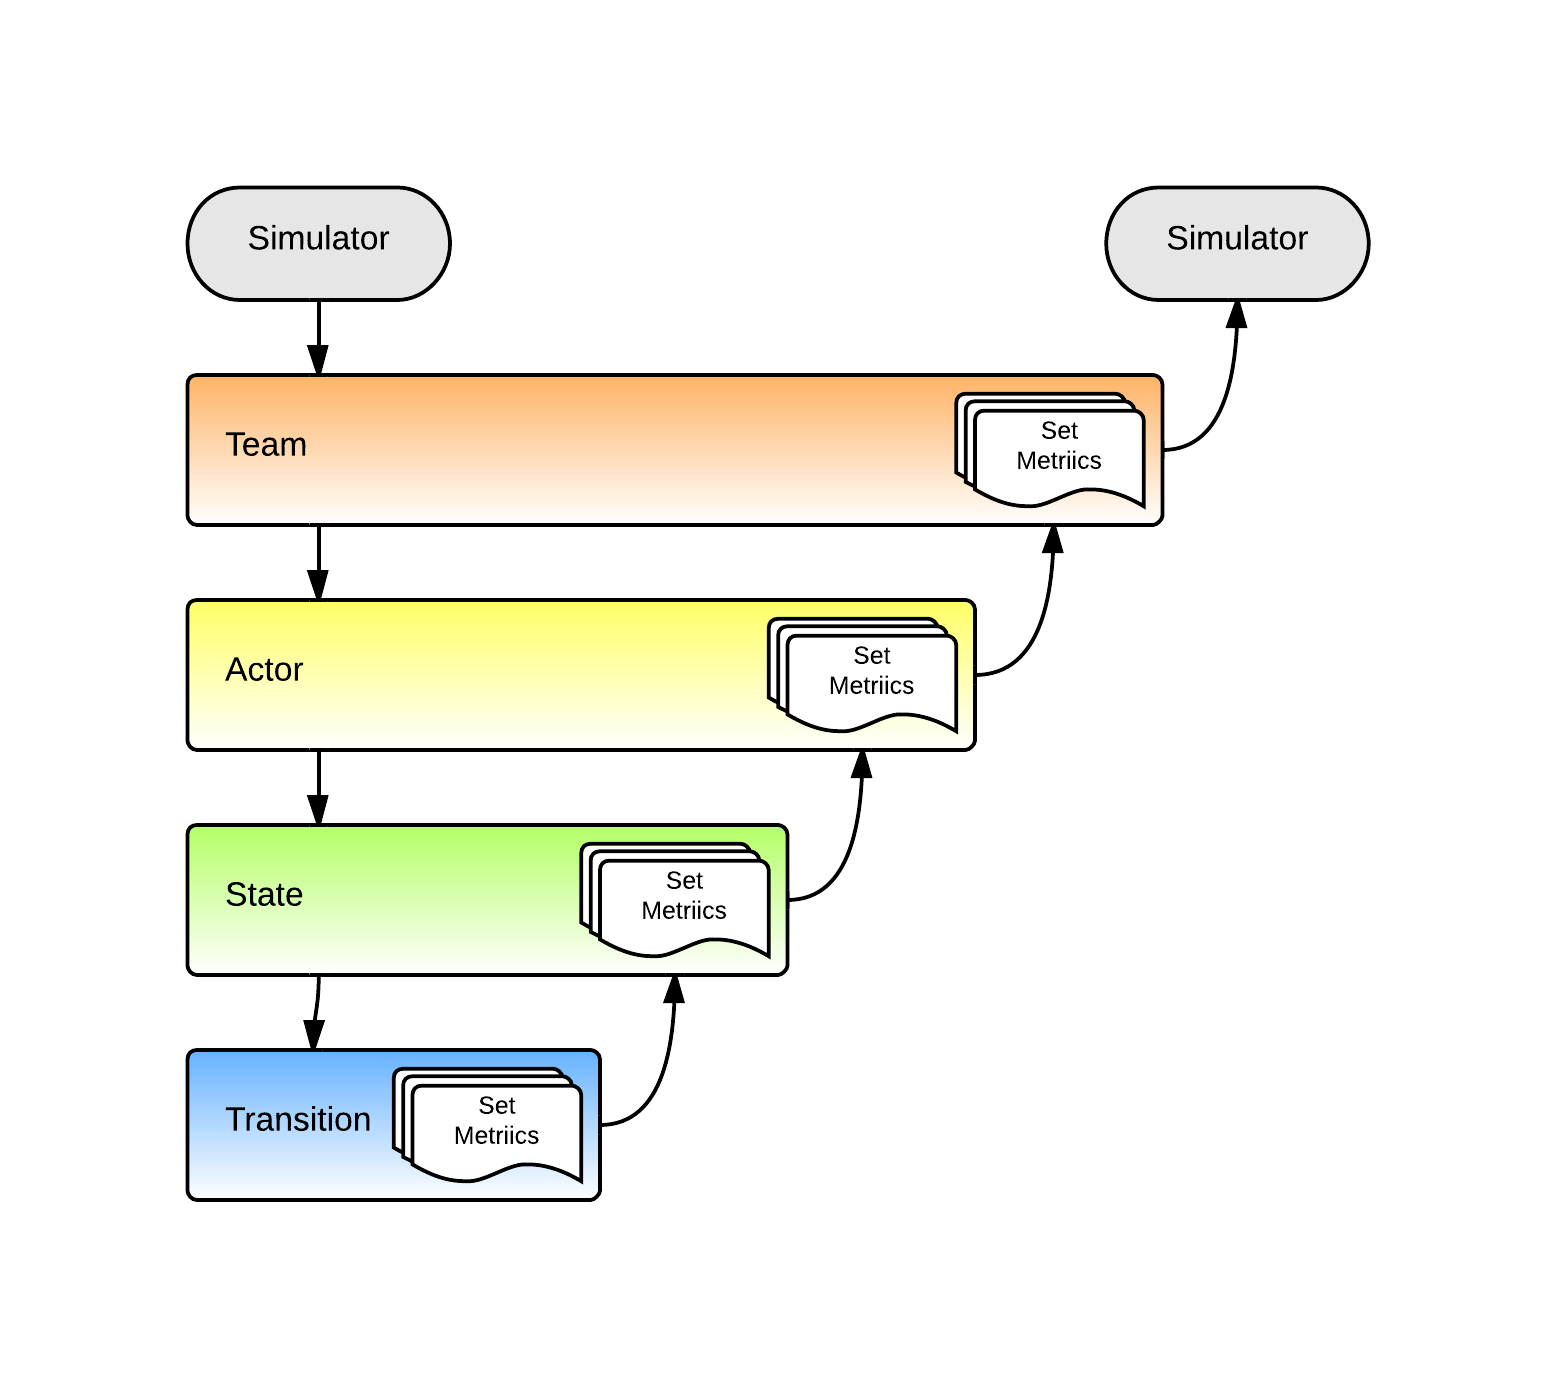
\includegraphics[width=6in]{metric_gathering.png}
\caption{Metric Gathering}
\label{fig:metric_gathering}
\end{center}
\end{figure}


We can see this in action by examining the Actor metric stack.  The Actor knows how many input channels he can listen on, his current state, etc.  The Actor does not directly know what transitions are enabled, how many inputs are in those transitions, etc.  Instead of trying to calculate all of this with multiple queries into the state the Actor simply asks the State object for its metrics.  The State then obtains/calculates metric values, obtaining metrics from sub-components if needed, before passing these values back to the Actor.  Once each Actor has returned a set of metrics, the Team returns these metrics in the form of an array.  The Simulator uses this metric array for storage, post processing, and user display.  Results presented in the next chapter show the value of presenting the metrics in a unified timeline.



\section{Wickens' Computational Model}

Given the ability to extract data from the model hierarchy as described in the previous section, we can translate this data into meaningful metrics.  Since we are interested in metrics which reveal human workload we have chosen to replicate Wickens' basic computational model~\ref{eq:wickens_model}, based on Multiple Resource Theory~\cite{wickens2002multiple}, using data gathered from the Model Abstraction Framework.  Later we will use this metric as a baseline to compare against our own metrics.  Wickens' model takes the task difficulty, ranging from 0 to 2 where 0 is automated and 2 is difficult, of two tasks and adds them together.  It then adds the number of dimensional conflicts between the tasks, max of 4, which gives a result between 0 and 8.

\begin{equation}
W(T_{d}^{1}, T_{d}^{2}) = \left\{ 
  \begin{array}{l l}
    T_{d} \in \{0,1,2\} & \quad \text{Task Difficulty}\\
    D_{c}(T_{d}^{1}, T_{d}^{2})\in \{0,1,2,3,4\} & \quad \text{Dimensional Conflicts}\\
    T_{d}^1 + T_{d}^2 + D_{c}(T_{d}^{1}, T_{d}^{2}) & \quad \text{Wickens' model}
  \end{array}
  \right.
  \label{eq:wickens_model}
\end{equation}


The difficulty with applying this model to our metrics is that we have removed the concept of tasks and replaced it with the notion of state and inputs.  The Model Abstraction Framework allows us to express tasks and other workload factors as resource, decision, and temporal elements by creating an Actor state and modeling input consumption and output generation of that state.  This is beneficial for modeling vague or unknown systems since the modeler can focus on the input and output rather than specific task sets.  Unfortunately this focus on resource, decision, and temporal elements does not distinguish between tasks.  Any tasks are represented solely by an Actors state, which may represent any number of tasks being performed, preventing a direct mapping from Wickens' model to our own. 


\subsection{Determining Task Difficulty}
In order to generate similar workload metrics as Wickens' model we needed a way to represent task difficulty (resource demand) in a similar fashion.  Using transition duration, the longer a task takes the more difficult it is, does not work because it prevents the modeler from placing an Actor into a long running simple task.  Inputs do not work since the data going over a channel do not always reflect resource demand, shown by a human's ability to tune out certain inputs.  Further examination revealed that we had no way to explicitly define an Actor's resource demand with the Model Abstraction Framework.  Wickens' model allows the modeler to subjectively set the task difficulty from their own experience and intuition.  While it is possible to implicitly define task difficulty from resource, decision, and temporal elements of the model we believe that Wickens' approach, allowing the modeler to subjectively define this value, will be more accurate.  To accomodate this we chose to add this subjective difficulty value to the Model Abstraction Framework under the label of Actor Load.


	
\subsection{Actor Load}
Actor Load represents an abstraction of the load an Actor is under while in a specific state.  Similar to Wickens' model, we have abstracted the Actor Load into an integer value ranging from 0-4.  An Actor Load of 0 represents little to no load on the actor.  These are automated or transitional states where the Actor is idle or has minimal contact with the system.  An Actor Load of 4 represents simultaneously performing multiple high difficulty tasks.  These are states where an Actor is pushed to the limit of their cognitive capabilities. Any value between 0 and 4 is some combination of task difficulty and the number of tasks being performed.  Actor Load is subjectively assigned to an Actors' state by the modeler.

\subsection{Determining Dimensional Conflicts}
To calculate the dimensionality of resource conflicts we need a way to determine when multiple tasks are being performed.  Since the Model Abstraction Framework does not define specific tasks we must find another method to approximate when multiple tasks are being performed.  We accomplish this by making the assumption that if an Actor has input from multiple sources then multiple tasks are being performed.

\begin{figure}[h]
\begin{center}
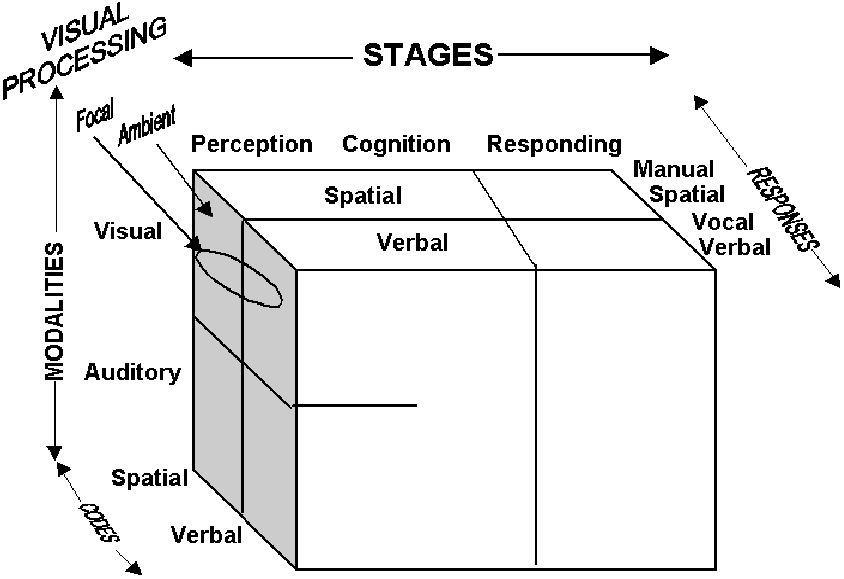
\includegraphics[width=6in]{multresourcetheory.png}
\caption{Multiple Resource Theory Dimensions}
\label{fig:multipleresourcetheory}
\end{center}
\end{figure}

With this assumption we are ready to calculate dimensional conflicts as illustrated in Figure~\ref{fig:multipleresourcetheory}.
For the Stage dimension (perception, cognition, response) we check to see if there are multiple sources of input or multiple targets for output.  If there are then we increment the dimensionality as shown in equation~\ref{eq:stage_dimension}.  

For the Modality dimension (Audio, Visual) we check if there is more than a single active channel, input or output, of type audio or visual.  If there is then we increment the dimensionality as shown in equation~\ref{eq:modality_dimension}.

For the Focus dimension we check if there is more than one target for tactile outputs, if there are then we increment the dimensionality as shown in equation~\ref{eq:focus_dimension}.  We do not check inputs as we have no way of distinguishing if a visual channel has focus.  This may need to be addressed in future work. 

For the Codes dimension (Spacial, Verbal) we check that the total number of audio inputs and outputs is greater than 1 or that the total number of visual inputs, visual outputs, and tactile outputs is greater than 1.  If either value is greater than 1 then we increment the dimensionality as shown in equation~\ref{eq:codes_dimension}.


\begin{equation}
D_{S}(Inputs, Outputs) = \left\{ 
  \begin{array}{l l}
    1, Inputs_{Sources} > 1 & \quad \text{Multiple Input Sources}\\
    1, Outputs_{Targets} > 1 & \quad \text{Multiple Output Targets}\\
    0, otherwise
  \end{array}
  \right.
  \label{eq:stage_dimension}
\end{equation}

\begin{equation}
D_{M}(Inputs, Outputs) = \left\{ 
  \begin{array}{l l}
    1, Inputs_{Active}^{Audio/Visual} > 1 & \quad \text{Multiple Active Inputs}\\
    1, Outputs_{Active}^{Audio/Visual} > 1 & \quad \text{Multiple Active Outputs}\\
    0, otherwise
  \end{array}
  \right.
  \label{eq:modality_dimension}
\end{equation}

\begin{equation}
D_{F}(Outputs) = \left\{ 
  \begin{array}{l l}
    1, Outputs_{Target}^{Tactile} > 1 & \quad \text{Multiple Tactile Output Targets}\\
    0, otherwise
  \end{array}
  \right.
  \label{eq:focus_dimension}
\end{equation}

\begin{equation}
D_{C}(Inputs, Outputs) = \left\{ 
  \begin{array}{l l}
    1, Inputs^{Audio} + Outputs^{Audio} > 1\\
    1, Inputs^{Visual/Tactile} + Outputs^{Visual/Tactile} > 1\\
    0, otherwise
  \end{array}
  \right.
  \label{eq:codes_dimension}
\end{equation}


\subsection{Adapted Wickens' Model}
Using the adaptations mentioned in this section we are able to replicate Wickens' model within the Model Abstraction Framework by summing the Actor Load with the dimensional conflict values.  See equation~\ref{eq:adapted_wickens_model}.  As the model values are calculated differently than Wickens' model we will refer to this model as an adapted Wickens' model.  We propose to use this adapted Wickens' model as a baseline comparison for our metrics since the core elements of the adapted Wickens' model are fundamentally the same as those in the original.  

\begin{equation}
W(ActorLoad, D_{S}, D_{M}, D_{F}, D_{C}) = \left\{ 
  \begin{array}{l l}
    ActorLoad \in \{0,1,2,3,4\}\\
    ActorLoad + D_{S} + D_{M} + D_{F} + D_{C}
  \end{array}
  \right.
  \label{eq:adapted_wickens_model}
\end{equation}


\section{Changes to our Metrics}
In addition to introducing an adapted Wickens' model we have also made improvements to the metric gathering presented in chapter 3.  The XML parser from the previous chapter builds each Actor, State, and Transition object from a unified set of Java classes.  By placing our metric gathering algorithms within these classes we are guaranteed to achieve the same metric gathering for all Actors.  We also have the ability to pre-process the metric values due to the new metric gathering process described earlier in the chapter.  By pre-processing the metrics within the original context we are better able to ensure that the metric values are more consistent with the theory.  

\subsection{Resource Workload Changes}
For the \textit{resource workload} category we now generate Actor metrics the following way.  Inputs are gathered from each transition that is part of the current state.  The outputs are collected from the active transition.  We also use the Actor load from the current state.  There are 2 main metrics: the channel conflicts and the resource load.  Channel conflicts occur whenever more than one active channel share a type, such as multiple audio channels.  Since we currently only allow visual and audio input for human Actors this value ranges from 0 to 2.  The other metric is the resource load.  This metric attempts to quantify the load being placed on the Actor's resources.  We break the resource load into two parts, input and output, the final result being the sum of both parts.  Each part is calculated by adding the number of active channels, number of layers read, number of memory objects read, and the number of active channel types.

\subsection{Decision Workload Changes}
For \textit{decision workload} we have added input complexity and output complexity.  The input complexity is the total number of active inputs plus the number of memory inputs.  The output complexity is the number of output channels plus the number of memory outputs.  While there is overlap between these values and the resource workload metrics we will leave it up to future work to analyze this relationship.  We have also modified the duration complexity metric.  Before adding Actor Load we relied on the duration complexity to inform us of task size by assuming that Actors performance does not vary across states.  This meant that if one state took longer than another it was because there was more work to be done.  We no longer make these assumptions about duration.  We have chosen to keep the duration metric and to normalize the value using a logarithmic scale.  By assuming that durations are in seconds we classify any transition under a minute as 0 complexity and move up from there.  While the diminishing returns of this model allow us to show the duration complexity within the context of our other metrics it does not account for human fatigue and other factors of long running tasks.  We leave it up to future work to determine the usefulness of duration complexity and how it should be calculated.

\subsection{Temporal Workload Changes}
No direct changes were made to the \textit{temporal workload} metrics from chapter 3.  As part of the XML Model Parser extension the connections to JPF were temporarily disabled to simplify the debugging process.  The results described in the next chapter were obtained by running the simulator as a stand alone application outside of JPF.  While this does prevent a deeper evaluation of the models state space the core model behavior still remains the same.  Unfortunately it prevented us from collecting the temporal workload metrics from the model.
